\documentclass[12pt,a4paper]{article}
\usepackage[spanish]{babel}
\usepackage[utf8]{inputenc}
\usepackage[T1]{fontenc}
\usepackage{geometry}
\usepackage{graphicx}
\usepackage{float}
\usepackage{booktabs}
\usepackage{hyperref}
\usepackage{tcolorbox}
\usepackage{siunitx}
\usepackage{caption}
\usepackage{subcaption}
\geometry{margin=2.5cm}
\sisetup{locale = FR, detect-all}
\graphicspath{{../imagenes/}}

\begin{document}

\begin{center}
    {\huge \bfseries Informe de Análisis de la Fuente}\\[4pt]
    {\Large \bfseries Placa "hijo" – Estación de calidad del aire}\\[8pt]
    \rule{0.9\textwidth}{1pt}\\[10pt]
\end{center}

\begin{figure}[H]
	\centering
	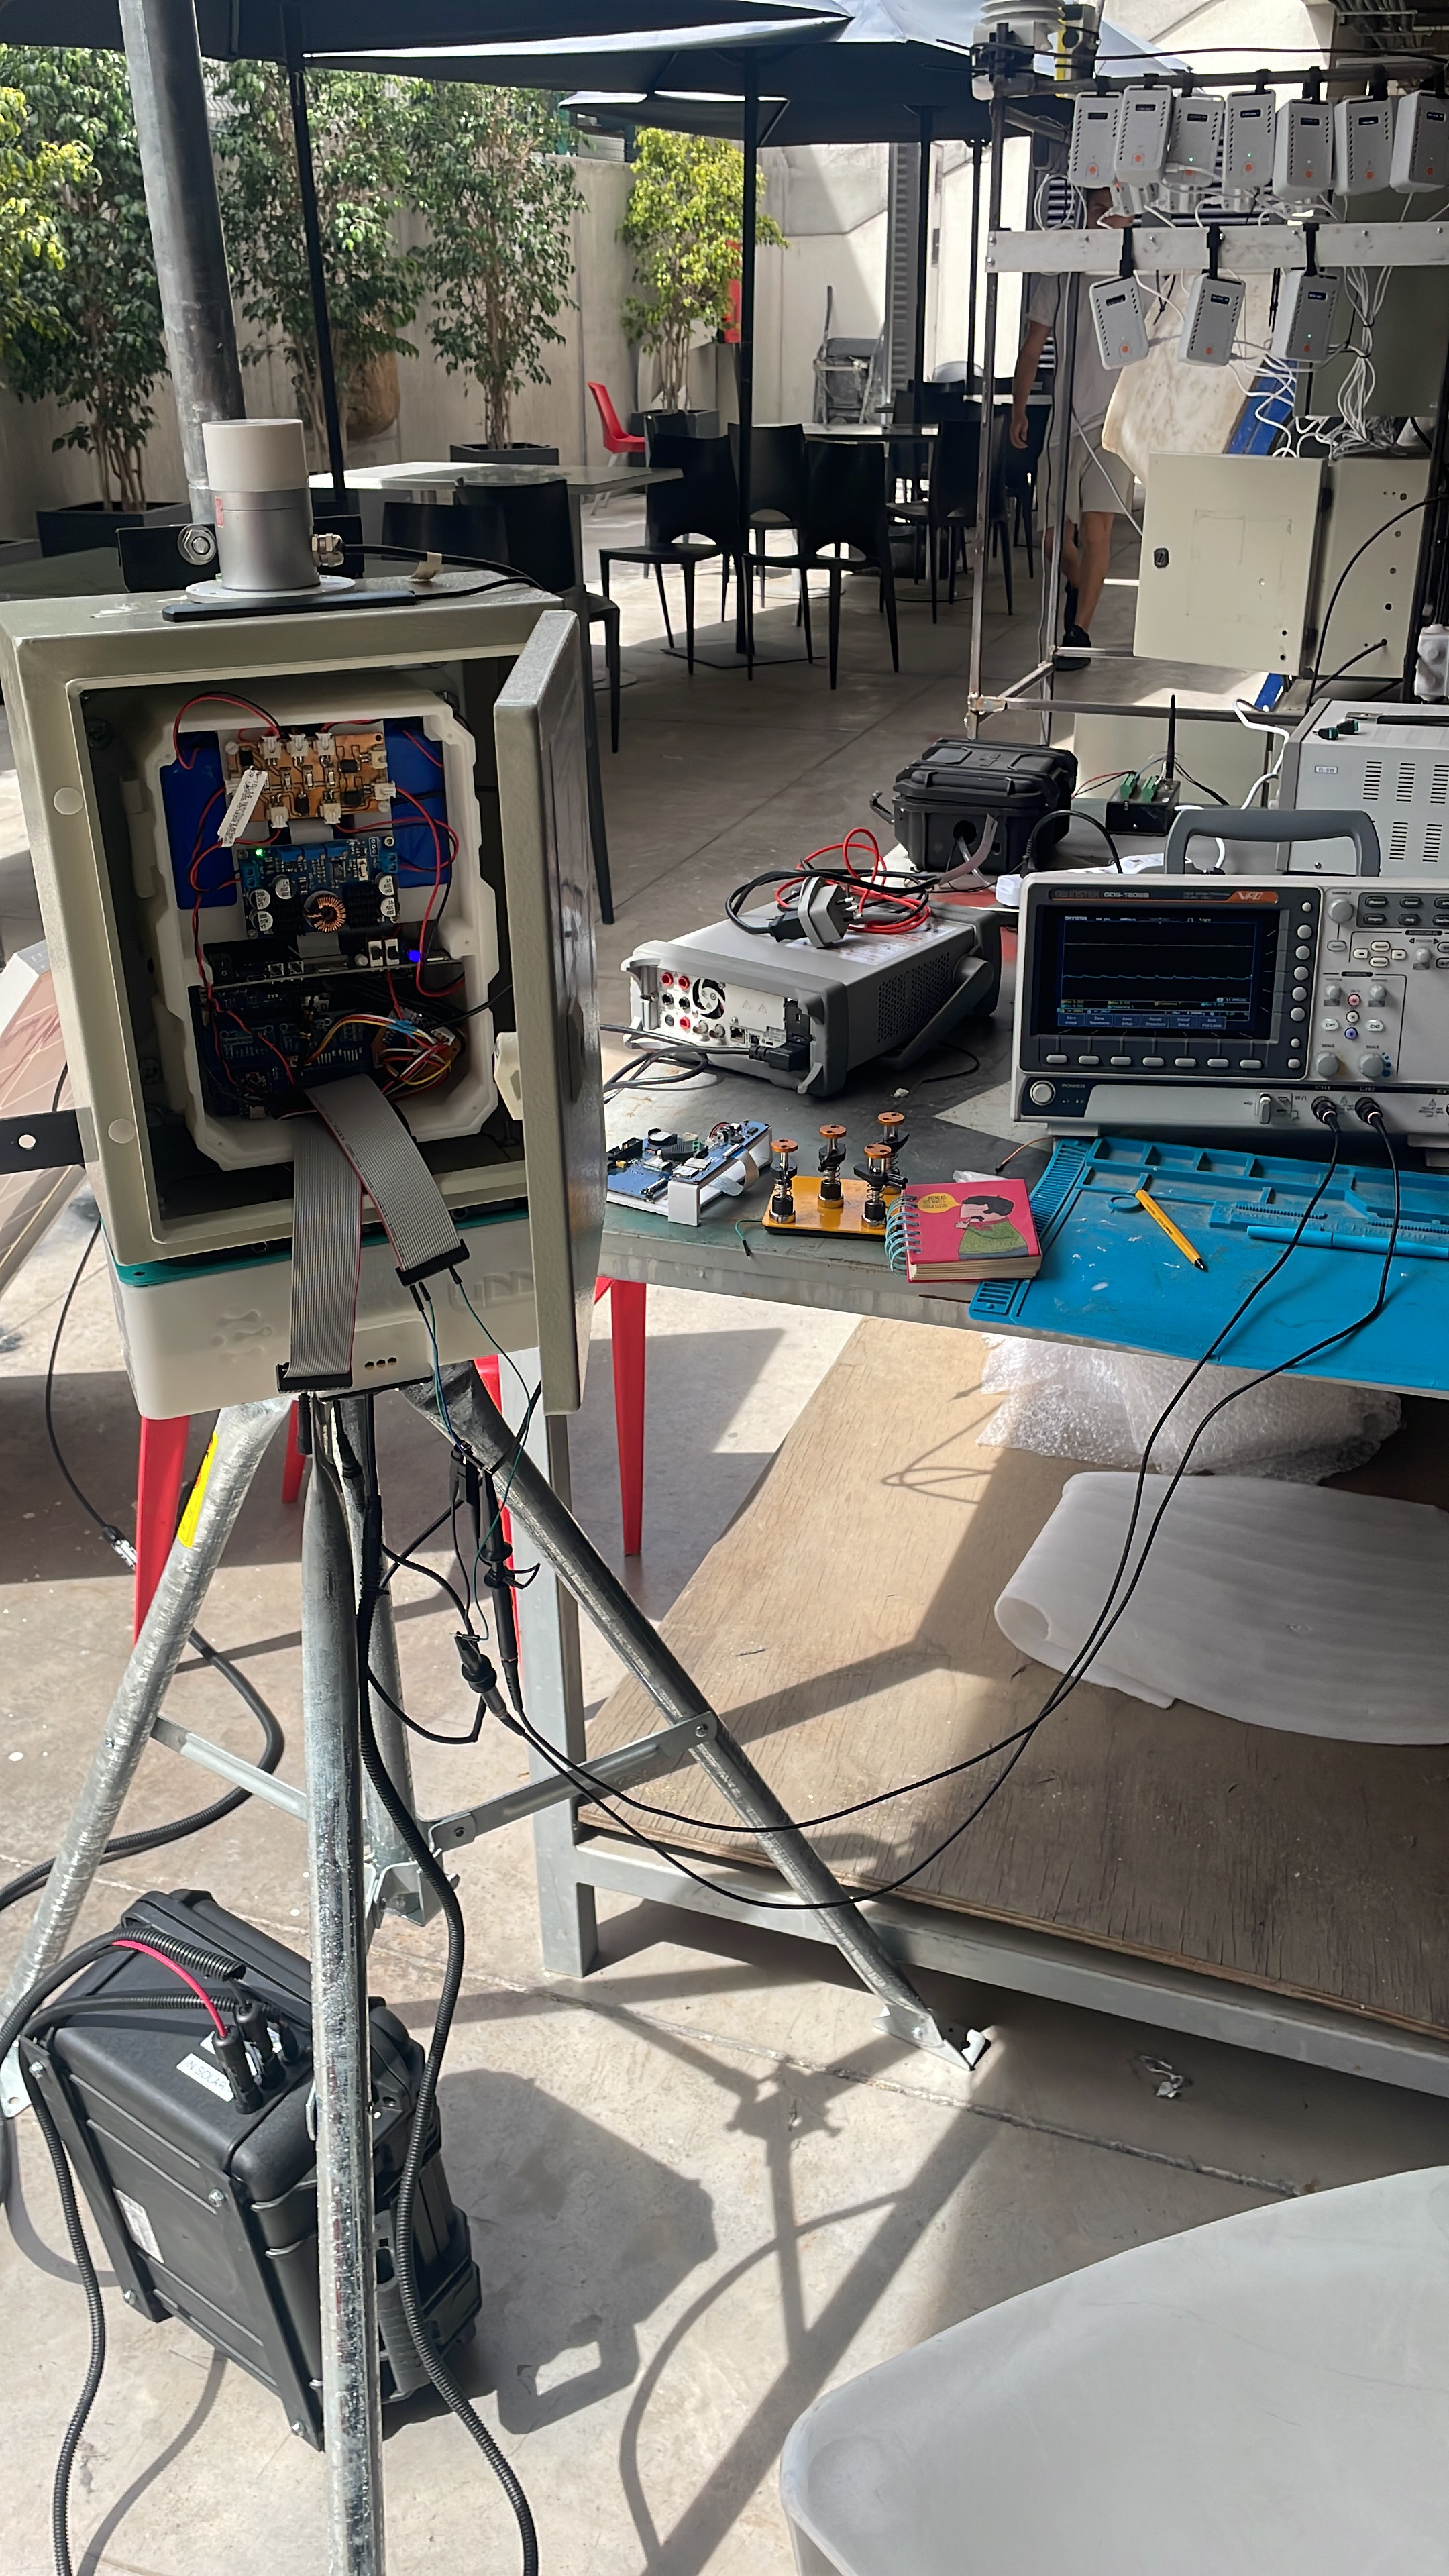
\includegraphics[width=0.5\linewidth]{prueba_fuente.jpg}
	\caption{Vista general del montaje de prueba.}
	\label{fig:montaje}
\end{figure}



\begin{tcolorbox}
    \textbf{Responsable:} Luis Gómez (\href{mailto:luis.gomez@udd.cl}{luis.gomez@udd.cl})\\
    \textbf{Revisores:} Alejandro Rebolledo (\href{mailto:arebolledo@udd.cl}{arebolledo@udd.cl})\\
    \textbf{Lugar:} Equipo transversal, Laboratorio C+ UDD, Santiago\\
    \textbf{Fecha:} 17 noviembre 2025 (14:00–16:00)\\
    \textbf{Estación evaluada:} Estación 1\\
    \textbf{Proyecto:} Línea base pública para la Región Metropolitana\\
\end{tcolorbox}

\section{Propósito del test}

El objetivo del ensayo fue verificar el desempeño de la fuente de alimentación de la estación de calidad del aire, medida en el cable IDC que alimenta a los sensores electroquímicos AlphaSense desde la placa denominada \textit{hijo}. Se buscó confirmar:
\begin{itemize}
    \item la correcta asignación de pines Vout (\SI{5}{\volt} y \SI{3.3}{\volt}) y GND en el conector IDC,
    \item la estabilidad temporal de las líneas de alimentación sin carga,
    \item el nivel de ruido instantáneo y la relación señal/ruido (S/R) disponible para los acondicionadores AlphaSense.
\end{itemize}

\section{Procedimiento}

\subsection*{Condiciones del ensayo}
\begin{itemize}
    \item Se mantuvo la Estación 1 en operación normal (panel solar y conjunto de baterías), alimentando la placa hijo y el cable paralelo.
    \item Se verificó con multímetro digital la continuidad y polaridad de Vout (\SI{5}{\volt} y \SI{3.3}{\volt}) y de GND antes de conectar las puntas del osciloscopio.
    \item Las mediciones dinámicas se realizaron con el cable conectado únicamente a los sensores electroquímicos, sin cargas adicionales, para capturar el ripple bajo las condiciones nominales de operación.
\end{itemize}

\begin{figure}[H]
    \centering
    \begin{subfigure}[b]{0.65\linewidth}
        \centering
        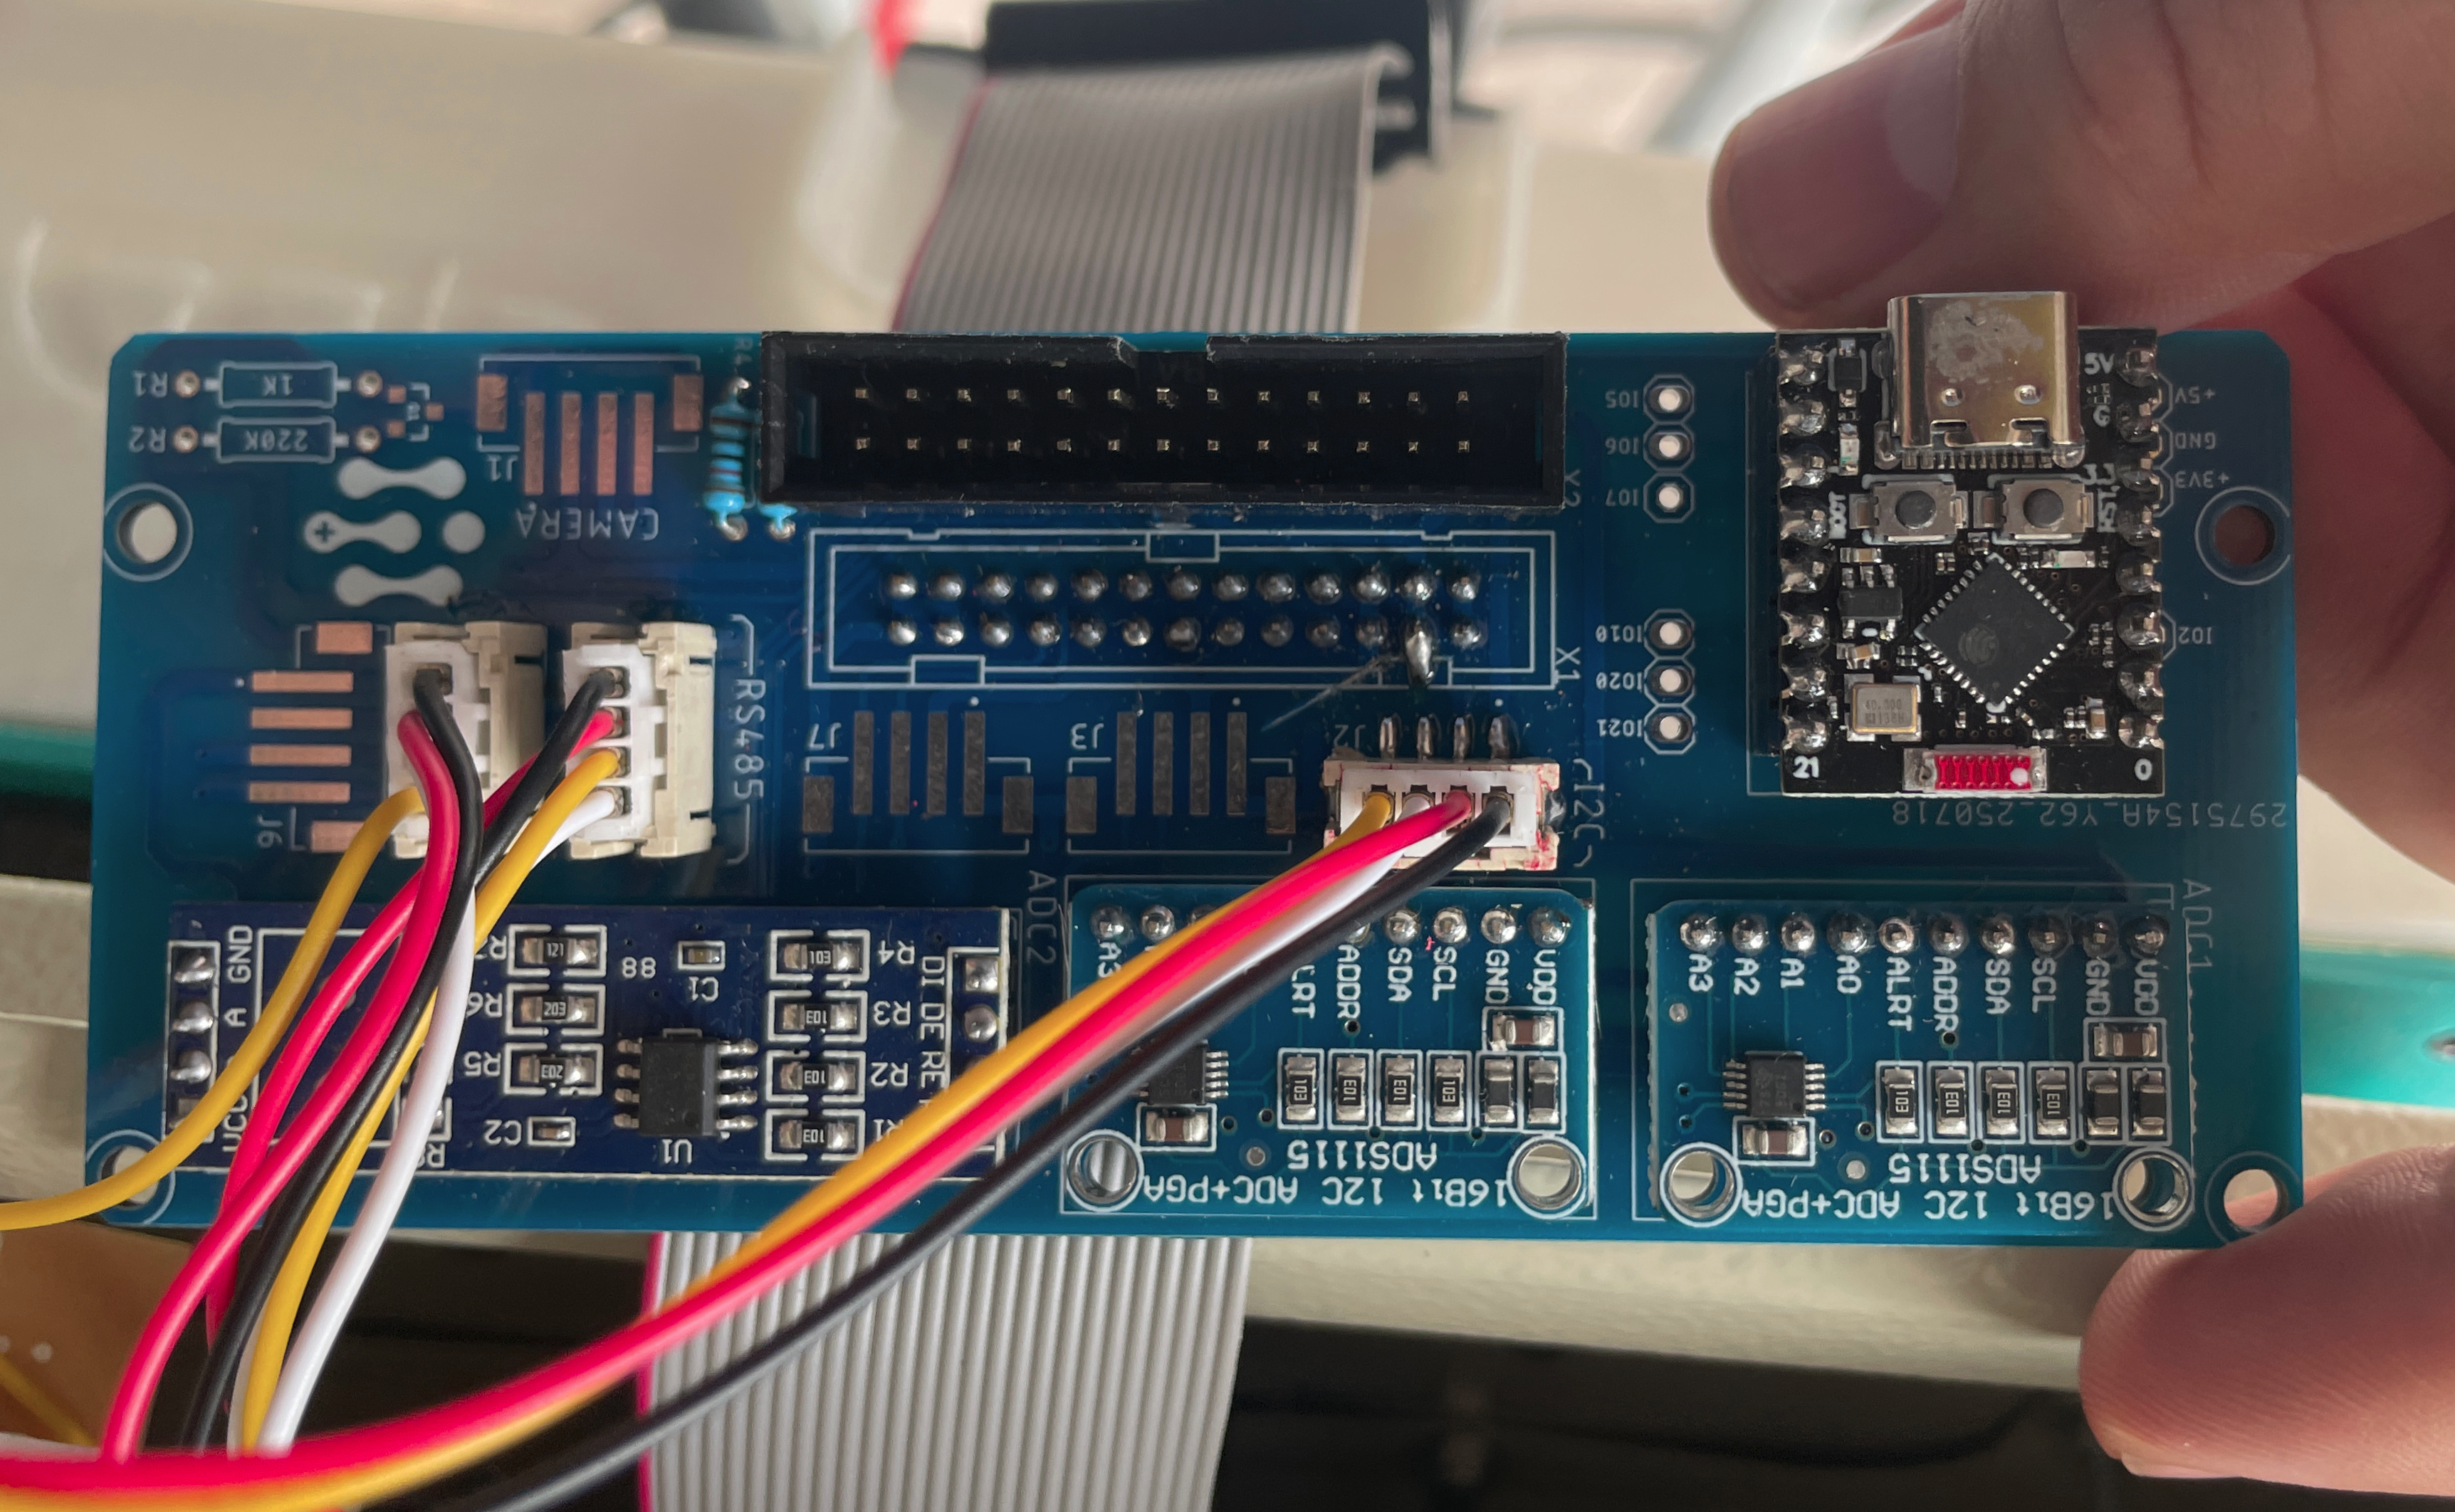
\includegraphics[width=\linewidth]{placa_hijo.png}
        \caption{Placa denominada hijo.}
        \label{subfig:placa-hijo}
    \end{subfigure}
    \hfill
    \begin{subfigure}[b]{0.3\linewidth}
        \centering
        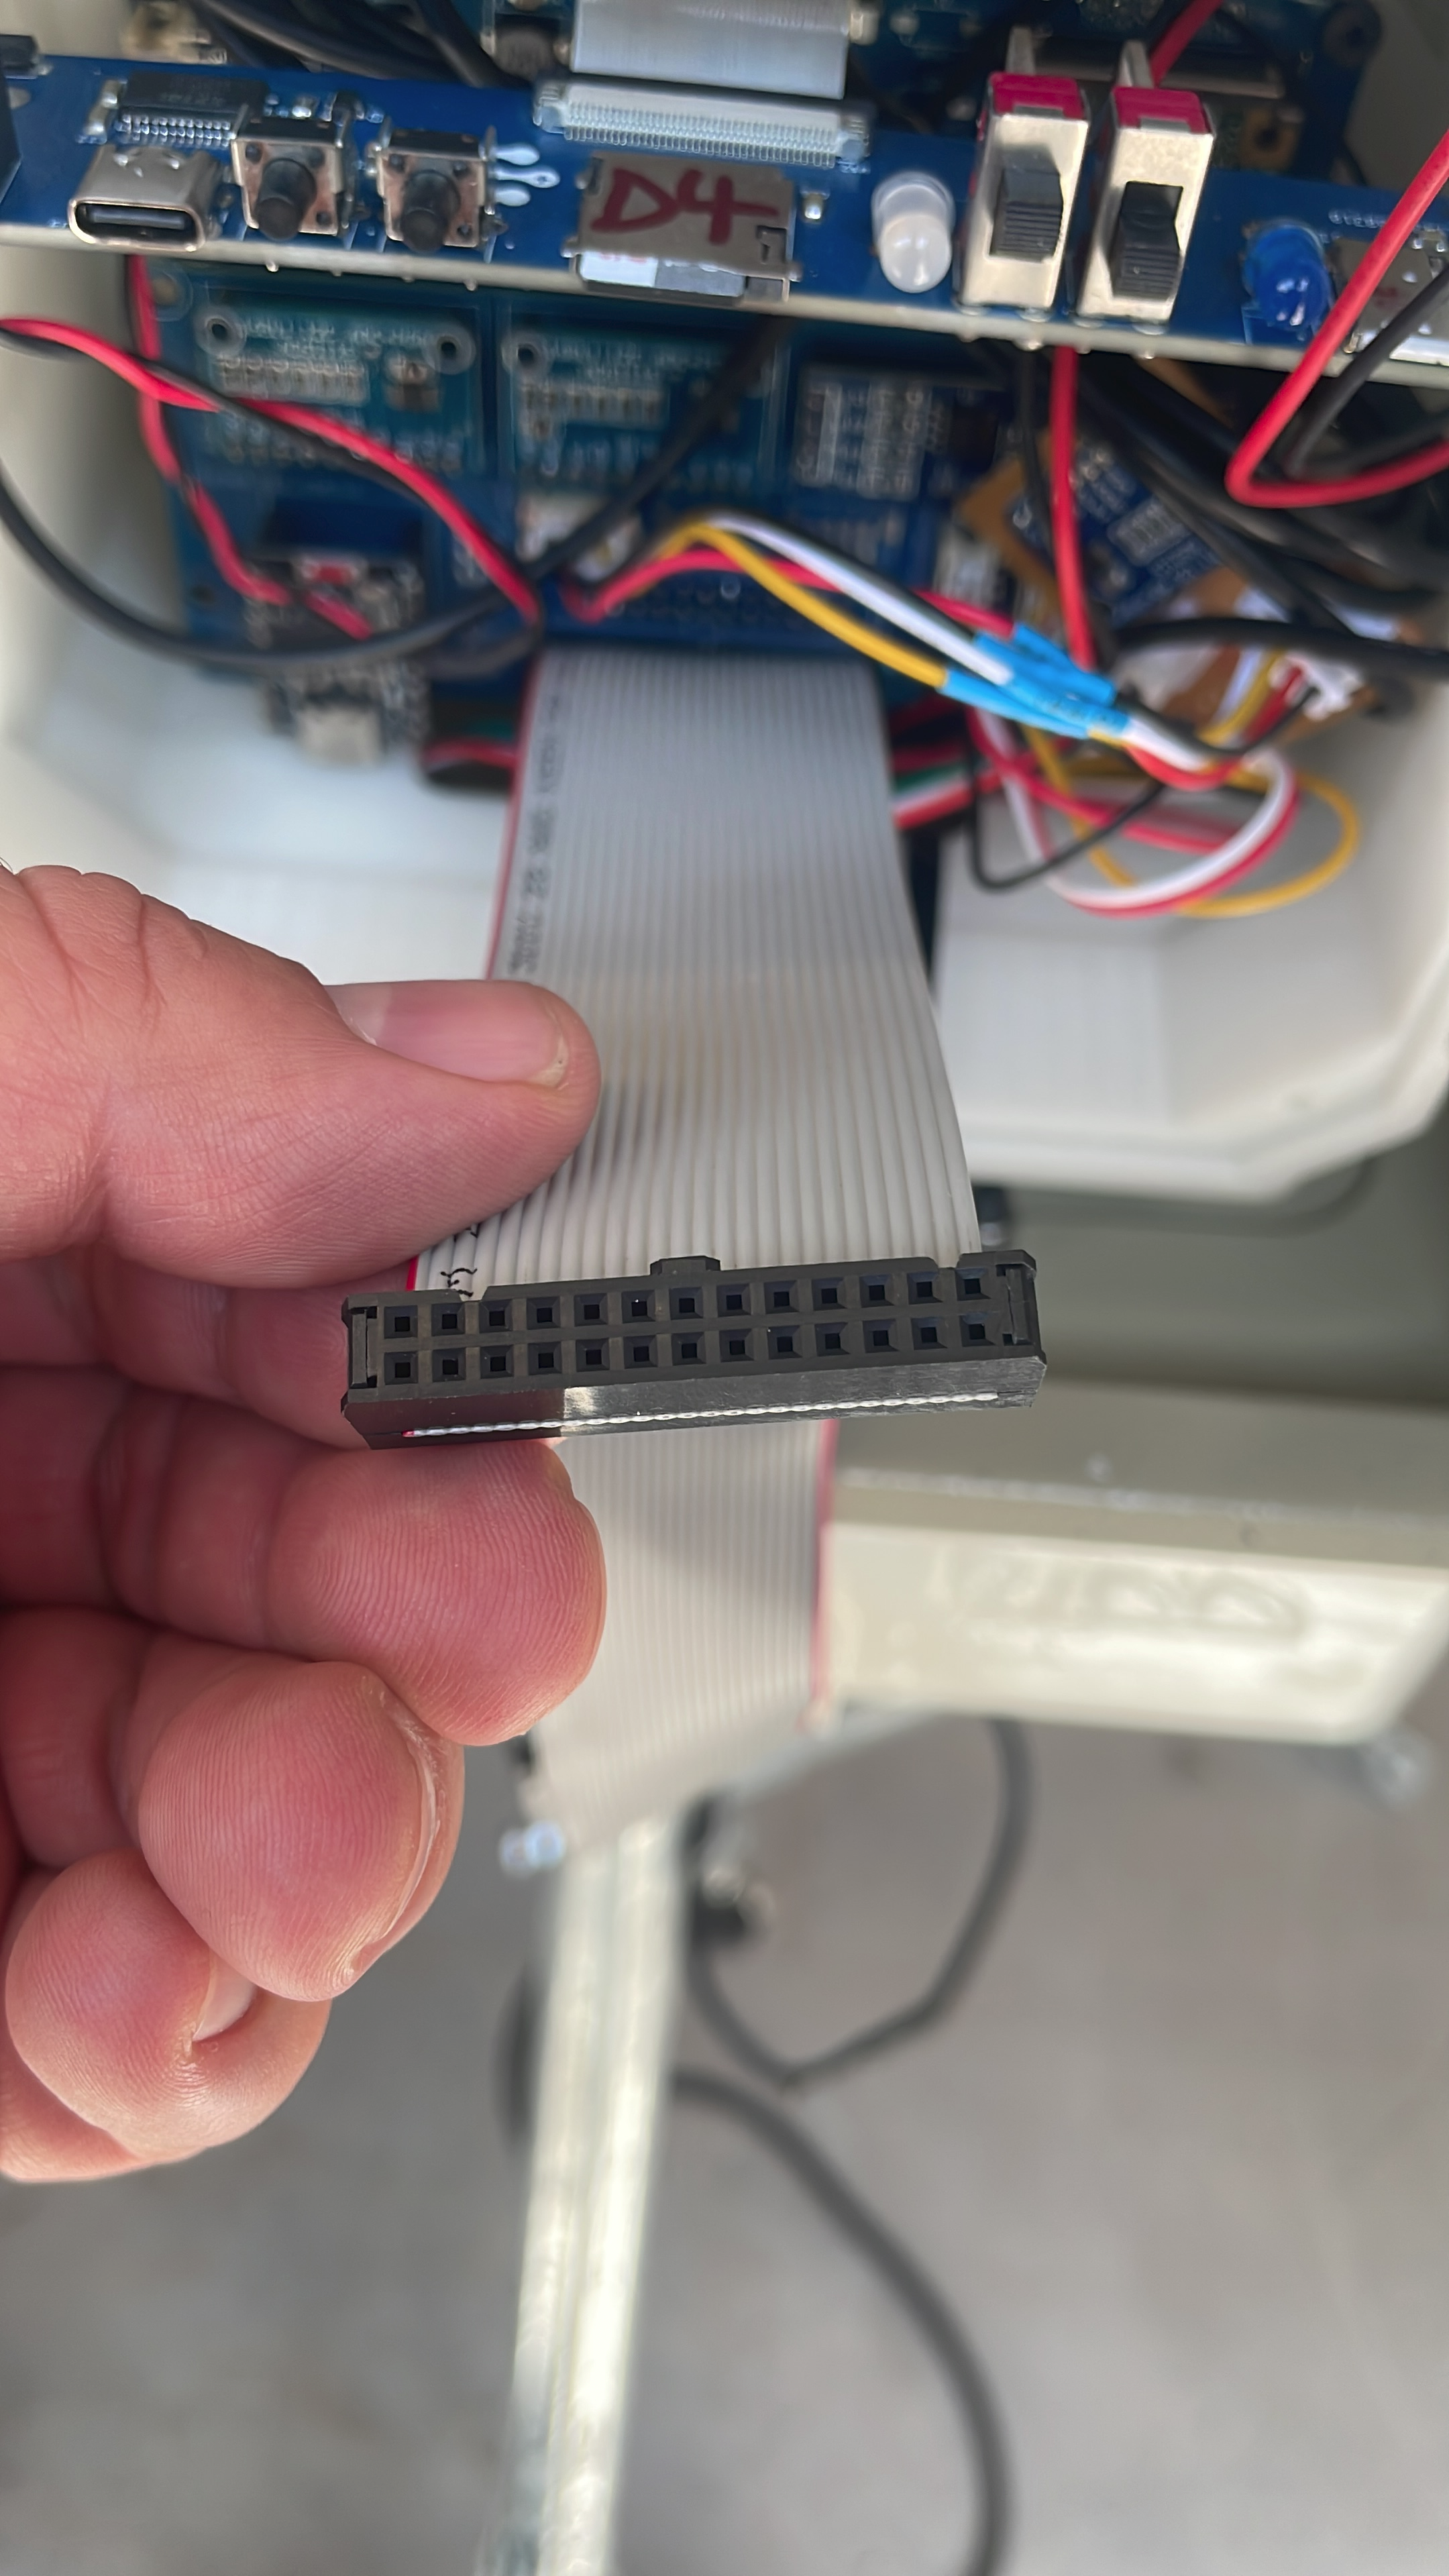
\includegraphics[width=\linewidth]{conector_IDC_hembra_sensores.png}
        \caption{Conector IDC hembra.}
        \label{subfig:idc}
    \end{subfigure}
    \caption{Puntos donde se verificaron Vout y GND antes de conectar el osciloscopio.}
    \label{fig:placahijo}
\end{figure}

\subsection*{Equipamiento}
\begin{itemize}
    \item Multímetro digital Keysight 34461A para verificación de pines.
    \item Osciloscopio GW Instek serie GDS (firmware V1.29) con puntas 1×.
    \item Computador portátil con software GW Instek para exportar los archivos CSV de 10.000 muestras.
\end{itemize}



\subsection*{Metodología de medición}

\begin{enumerate}
    \item Identificación con multímetro de los pines Vout (\SI{5}{\volt}, \SI{3.3}{\volt}) y GND para garantizar continuidad y polaridad adecuadas.
    \item Conexión de las puntas del osciloscopio directamente en el conector IDC del cable paralelo, asegurando la referencia común.
    \item Captura de dos ventanas de 10.000 muestras por canal, almacenadas en los archivos \texttt{DS0003.CSV} (\SI{3.3}{\volt}) y \texttt{DS0004.CSV} (\SI{5}{\volt}).
    \item Procesamiento estadístico (mínimo, máximo, promedio, desviación estándar y S/R) mediante Python para cada traza.
\end{enumerate}


\begin{figure}[H]
    \centering
    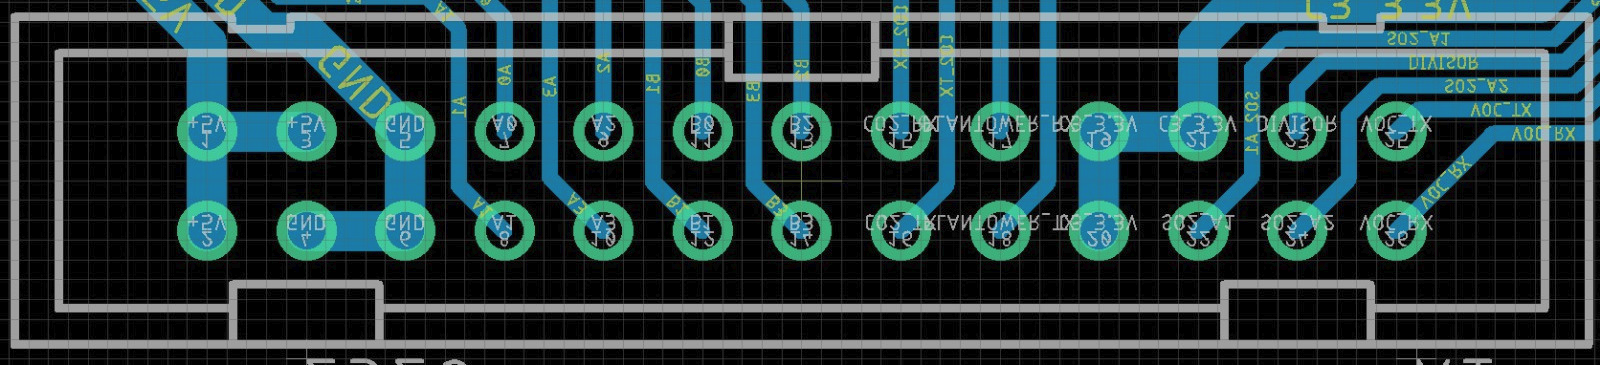
\includegraphics[width=0.7\linewidth]{conectores_paralelo_alimentacion_datos_sensores.png}
    \caption{Distribución de conectores del cable paralelo que llega a los sensores.}
    \label{fig:conectores}
\end{figure}

\section{Resultados}

Los datos exportados permiten resumir el comportamiento de las líneas de alimentación según la Tabla~\ref{tab:resultados}. La desviación estándar corresponde al ruido RMS de la señal y se emplea para calcular la relación señal/ruido S/R.

\begin{table}[H]
    \centering
    \caption{Resultados estadísticos obtenidos de los archivos del osciloscopio.}
    \label{tab:resultados}
    \begin{tabular}{lcccccc}
        \toprule
        \textbf{Línea} & \textbf{Archivo} & $V_{\min}$ (V) & $V_{\max}$ (V) & $V_{\text{ave}}$ (V) & $\sigma$ (V) & \textbf{S/R}\\
        \midrule
        Vout \SI{3.3}{\volt} & \texttt{DS0003.CSV} & 3.250 & 3.260 & 3.259998 & 0.000141 & 2.31$\times 10^4$\\
        Vout \SI{5}{\volt} & \texttt{DS0004.CSV} & 5.120 & 5.180 & 5.142737 & 0.010890 & 4.72$\times 10^2$\\
        \bottomrule
    \end{tabular}
\end{table}

En la Figura~\ref{fig:osciloscopio} se aprecia las forma de ondas correspondientes a la línea de \SI{5}{\volt} (linea turqueza) y \textbf{3.3}{\volt}, donde se observa un rizado periódico de pequeña amplitud superpuesto al valor continuo de la fuente. El comportamiento es consistente con el ripple típico generado por convertidores DC--DC bajo carga ligera. 

\begin{figure}[H]
	\centering
	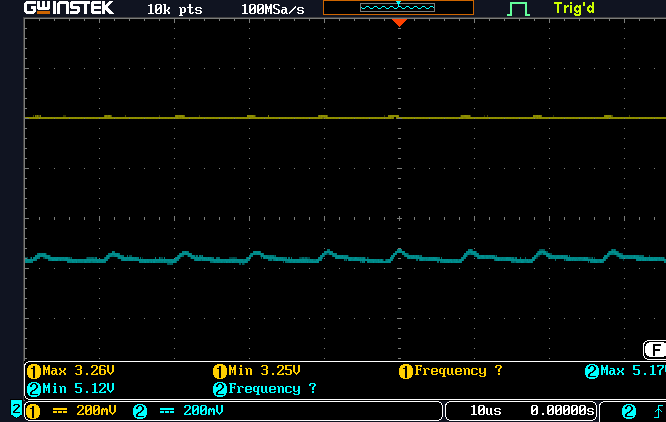
\includegraphics[width=0.75\linewidth]{medicion_osciloscopio_fuente.png}
	\caption{Captura del osciloscopio GW Instek GDS durante la caracterización de rizado en las líneas de \SI{3.3}{\volt} y \SI{5}{\volt}.}
	\label{fig:osciloscopio}
\end{figure}




La oscilación presenta un valor mínimo cercano a \SI{5.12}{\volt} y un máximo alrededor de \SI{5.17}{\volt}, lo que implica un rizado del orden de \SI{50}{\milli\volt} pico a pico. Esta magnitud se encuentra dentro de los rangos esperados para la etapa de alimentación de la estación y no representa un riesgo para la operación de los módulos AlphaSense, cuyo acondicionamiento analógico es tolerante a variaciones de este nivel.

La estabilidad general de la señal y la ausencia de caídas bruscas indican que no existen falsos contactos ni pérdidas transitorias en el cableado IDC. En consecuencia, la fuente mantiene un comportamiento adecuado para la operación del sistema.




\subsection{Análisis temporal y espectral del rizado en 5 V}

En la Figura~\ref{fig:ripple5V_tiempo} se muestra la forma de onda del riel de \SI{5}{\volt} obtenida a partir de 10.000 muestras del archivo \texttt{DS0004.CSV}. Se observa un rizado periódico de baja amplitud superpuesto al nivel DC, consistente con el comportamiento esperado de un convertidor DC--DC en régimen estable.

\begin{figure}[H]
	\centering
	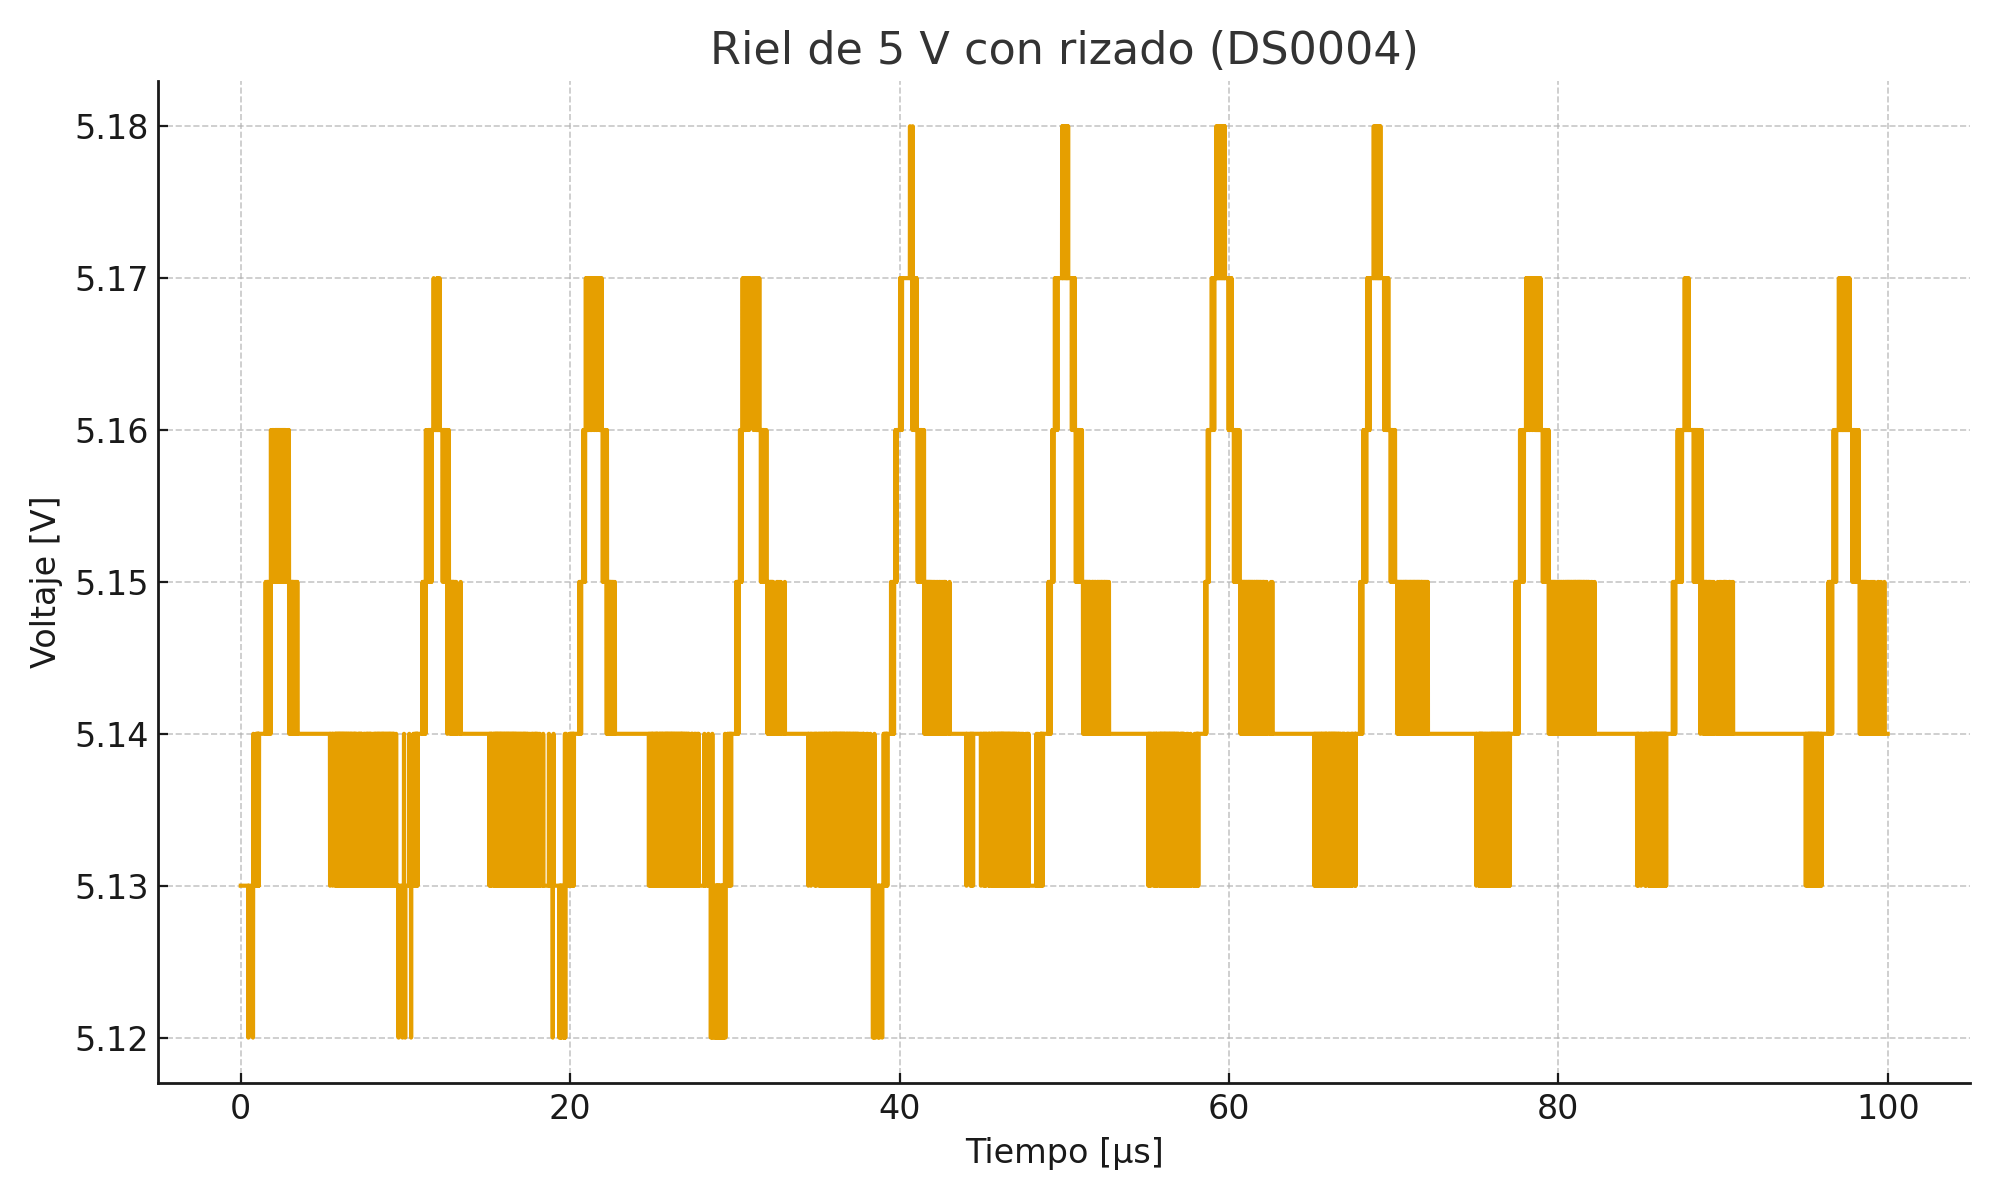
\includegraphics[width=0.85\linewidth]{../graficos/ripple_5V_tiempo.png}
	\caption{Forma de onda del riel de \SI{5}{\volt} obtenida desde el archivo \texttt{DS0004.CSV}. Se observa el rizado periódico superpuesto al nivel DC.}
	\label{fig:ripple5V_tiempo}
\end{figure}

Para caracterizar su contenido frecuencial se aplicó una FFT sobre la señal centrada (se restó el valor medio y se utilizó una ventana de Hann). El espectro resultante se presenta en la Figura~\ref{fig:ripple5V_fft}, donde se identifica un pico dominante en torno a los \SI{110}{\kilo\hertz}. Esta frecuencia es coherente con la frecuencia de conmutación típica de los reguladores conmutados utilizados en este tipo de fuentes.

\begin{figure}[H]
	\centering
	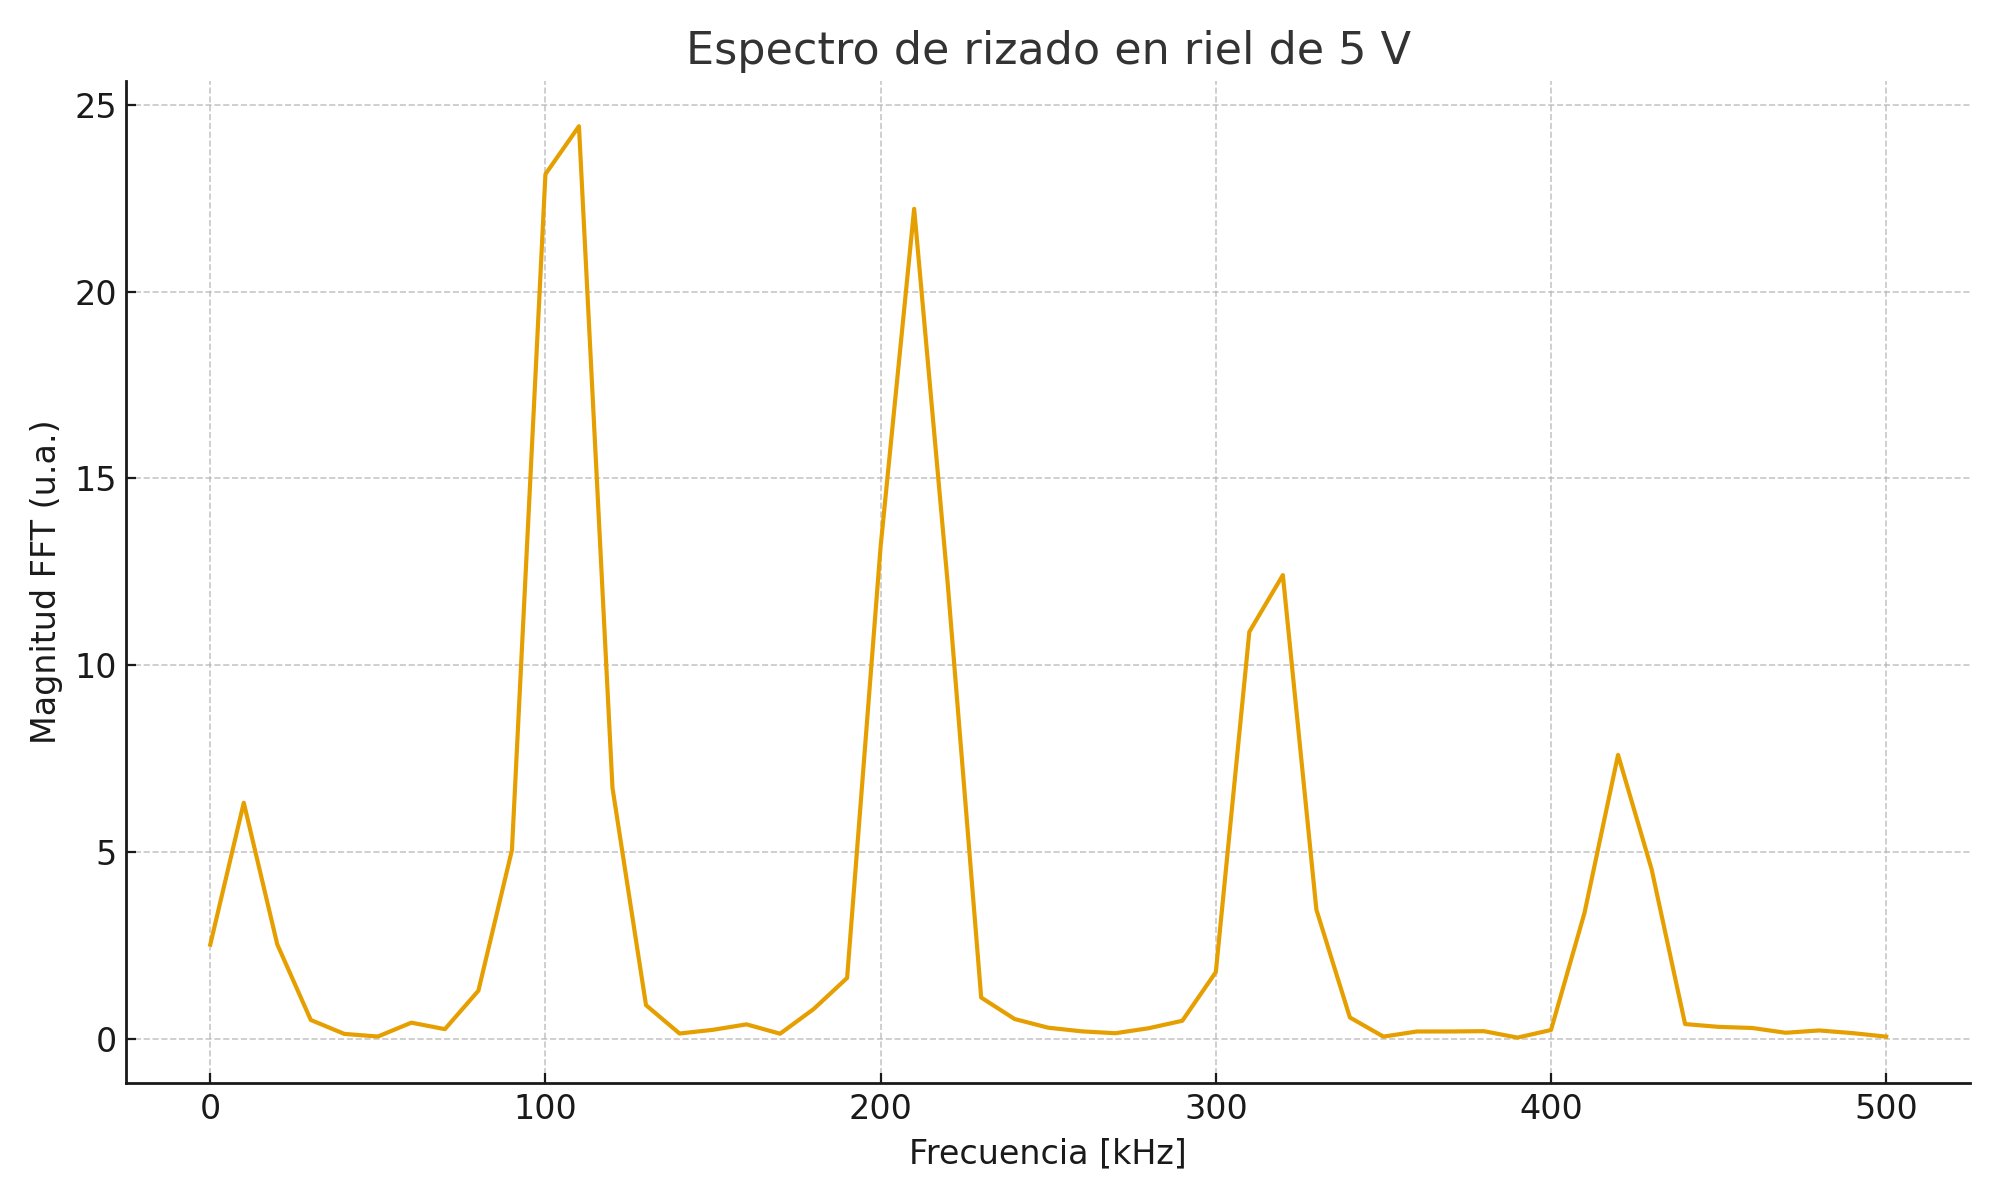
\includegraphics[width=0.85\linewidth]{../graficos/ripple_5V_fft.png}
	\caption{Espectro de amplitud del riel de \SI{5}{\volt} calculado mediante FFT a partir de 10.000 muestras (archivo \texttt{DS0004.CSV}).}
	\label{fig:ripple5V_fft}
\end{figure}



La amplitud del rizado en el dominio del tiempo es del orden de \SI{60}{\milli\volt} pico a pico, mientras que su componente fundamental se concentra en torno a \SI{110}{\kilo\hertz}, por lo que su impacto sobre la banda útil de los sensores electroquímicos y del ADC es mínimo y puede ser atenuado adicionalmente mediante filtrado pasa--bajo y condensadores de desacople locales.


\subsection*{Observaciones}
\begin{itemize}
    \item La línea de \SI{3.3}{\volt} presenta un ruido RMS de solo \SI{0.141}{\milli\volt} con una relación S/R superior a 23.000, lo que demuestra la estabilidad requerida por la electrónica digital de los sensores.
    \item La línea de \SI{5}{\volt} muestra un rizado de \SI{60}{\milli\volt} pico a pico y un ruido RMS de \SI{10.9}{\milli\volt}; los valores permanecen dentro de las tolerancias de AlphaSense para excitación analógica.
    \item No se identificaron pulsos o caídas atribuibles a falsos contactos en el cable; la variación observada corresponde al ripple natural de la fuente bajo carga.
\end{itemize}

\section{Análisis}

Las mediciones confirman que ambas líneas alimentan correctamente a los módulos AlphaSense. La dispersión mínima de \SI{3.3}{\volt} indica una referencia limpia para los circuitos digitales y de comunicación. El riel de \SI{5}{\volt} exhibe un ripple contenido que se mantiene por debajo de \SI{\pm 0.6}{\percent} del valor nominal y no debería  introducir variaciones apreciables sobre la señal útil de los sensores.

La disponibilidad de los archivos CSV y el script de reprocesamiento permite repetir el análisis rápidamente ante futuras intervenciones o auditorías.

\section{Conclusiones}

\begin{itemize}
    \item El cable paralelo asociado a la placa hijo cumple con las especificaciones de tensión y ruido establecidas por AlphaSense para alimentar sensores electroquímicos. Durante la prueba no se identificaron interferencias.
    \item El ruido medido (\textless\SI{11}{\milli\volt} RMS) resulta insuficiente para afectar la linealidad de los acondicionadores o la lectura de los ADC conectados.
    \item No se detectaron problemas de continuidad ni de polaridad, por lo que el cable puede mantenerse en servicio en la Estación 1.
\end{itemize}

\section{Recomendaciones}

	\begin{tcolorbox}
	\textbf{Para asegurar la calidad de las mediciones:}
	\begin{itemize}
		\item Reducir la distancia entre el sensor y el ADC, y asegurar el blindaje de cables y componentes, conectándolos adecuadamente a tierra.
		\item Verificar la existencia y continuidad de los planos de tierra en las placas, especialmente en las zonas cercanas al acondicionamiento analógico.
		\item Incorporar filtros pasa–bajo mediante capacitores de desacople de 10\,nF y 100\,nF ubicados lo más próximos posible al conector Molex ISB.
	 \end{itemize}

    \textbf{Para futuros ensayos se recomienda:}
    \begin{itemize}
        \item repetir la captura de datos tras cualquier intervención en el cable o sensores para mantener un historial actualizado,
        \item realizar medición general pero con carga. Es decir con los sensores conectados.
        \item complementar el análisis con mediciones espectrales del ruido cuando se integren nuevos módulos AlphaSense,
        \item documentar mediante fotografías adicionales los detalles de conexión y cualquier modificación de hardware.
    \end{itemize}

\end{tcolorbox}



\begin{thebibliography}{9}
\bibitem{AlphasenseManual} Alphasense Ltd., \emph{4-Electrode Individual Sensor Board (ISB) User Manual}, Issue 7, 2019.
\bibitem{GWInstek} GW Instek, \emph{GDS-1000 Series Digital Oscilloscopes – User Manual}, 2021.
\end{thebibliography}

\end{document}
